\documentclass{beamer}
\usepackage[british]{babel}
\usepackage[utf8]{inputenc}
\usepackage{graphicx,hyperref,ucr_eie,url}
\usepackage{mdframed}
\usepackage{tikz}
\usetikzlibrary{snakes}
\usepackage{chronology}
\usepackage{listings}
\graphicspath{{../multimedia/images/}}
\definecolor{shadecolor}{RGB}{250,250,250}		%%boxes color
\lstset{
		basicstyle=\ttfamily,
		keywordstyle=\color{black},
		commentstyle=\color{black},
		stringstyle=\color{black},
		tabsize=2,
		backgroundcolor=\color{shadecolor}}

% The title of the presentation:
%  - first a short version which is visible at the bottom of each slide;
%  - second the full title shown on the title slide;
\title[Visual Communication]{Visual Communication with Technology} 

% Optional: a subtitle to be dispalyed on the title slide
%\subtitle{}

% The author(s) of the presentation:
%  - again first a short version to be displayed at the bottom;
%  - next the full list of authors, which may include contact information;
\author[Grupo - Renekton]{
  Francisco Mata Marín\\
  Jose Pablo Apú Picado\\
  Sebastian Ramírez Solano\\\medskip
  %{\small \url{p.vullers@cs.ru.nl}} \\ 
  %{\small \url{http://www.cs.ru.nl/~pim/}}}
  }

% The institute:
%  - to start the name of the university as displayed on the top of each slide
%    this can be adjusted such that you can also create a Dutch version
%  - next the institute information as displayed on the title slide
\institute[University of Costa Rica]{
  Electrical Engineering School \\
  IE-0117 - Programación Bajo Plataformas Abiertas}

% Add a date and possibly the name of the event to the slides
%  - again first a short version to be shown at the bottom of each slide
%  - second the full date and event name for the title slide
\date[\today]{
  2nd Development Project \\
  \today}

\begin{document}

\begin{frame}
  \titlepage
\end{frame}

\begin{frame}
  \frametitle{Outline}
  \tableofcontents
\end{frame}

% Section titles are shown in at the top of the slides with the current section 
% highlighted. Note that the number of sections determines the size of the top 
% bar, and hence the university name and logo. If you do not add any sections 
% they will not be visible.
%%*****************************************************************************
\section{Introduction}

\begin{frame}
\frametitle{Objectives}
\begin{itemize}
\item Introduce another way to interact with machines, using opencv and c++.
\item Implement computer vision to play a simple game.
\item Create passwords with gestures recognition.
\end{itemize}
\end{frame}
%%*****************************************************************************
\begin{frame}
\frametitle{Justification}
\begin{itemize}
\item Make the eviroment more interactive. 
\item Computer Vision is getting used by lots of people.  
\end{itemize}
\end{frame}
%%*****************************************************************************
\section{Requirements}

\begin{frame}
\frametitle{Hardware}
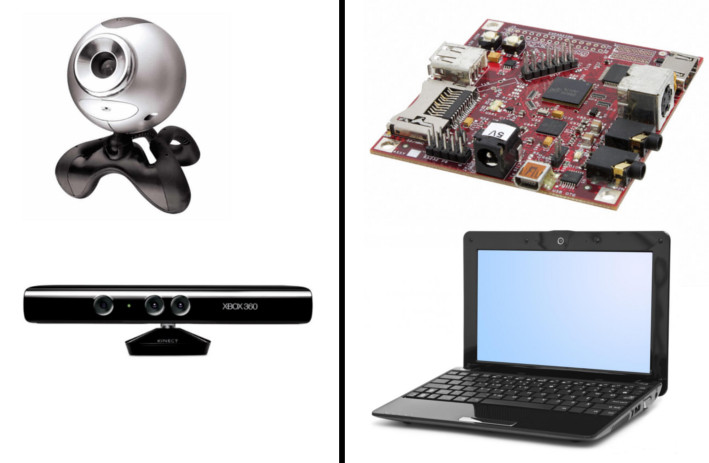
\includegraphics[scale=0.4]{requirements_hardware.jpg}
\end{frame}
%%*****************************************************************************
\begin{frame}
\frametitle{Software}
\begin{center}
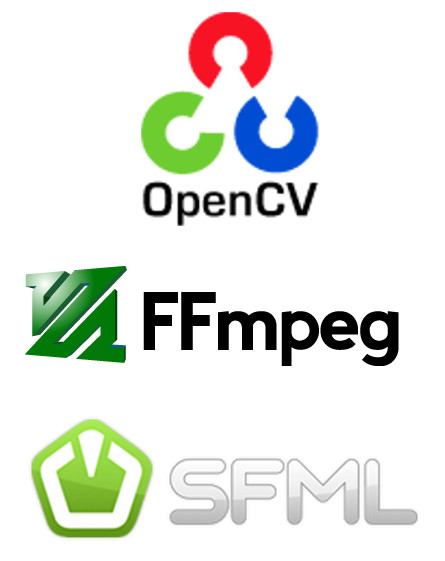
\includegraphics[scale=0.3]{requirements_libs.jpg}
\end{center}
\end{frame}
%%*****************************************************************************
\section{Computer Vision}
\begin{frame}
\frametitle{Main concepts}
Is a field that includes methods for acquiring, processing, analyzing, and understanding images and, in general, high-dimensional data from the real world in order to produce numerical or symbolic information,
\end{frame}
%%*****************************************************************************
\begin{frame}
\frametitle{Computer vision Methodes}
\begin{itemize}
\item Image acquisition
\item Pre-processing
\item Detection/segmentation
\item High-level processing
\end{itemize}
\end{frame}
%%*****************************************************************************
\begin{frame}
\frametitle{Image acquisition}
\begin{center}
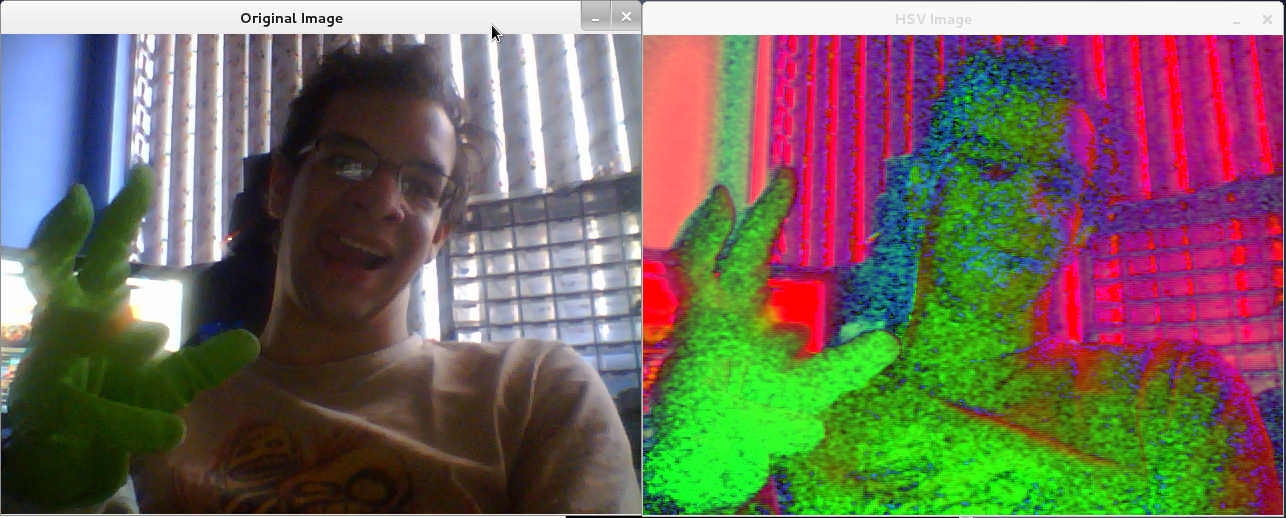
\includegraphics[scale=0.25]{pic01.png}
\end{center}
\end{frame}
%%*****************************************************************************
\begin{frame}
\frametitle{Pre-processing}
\begin{center}
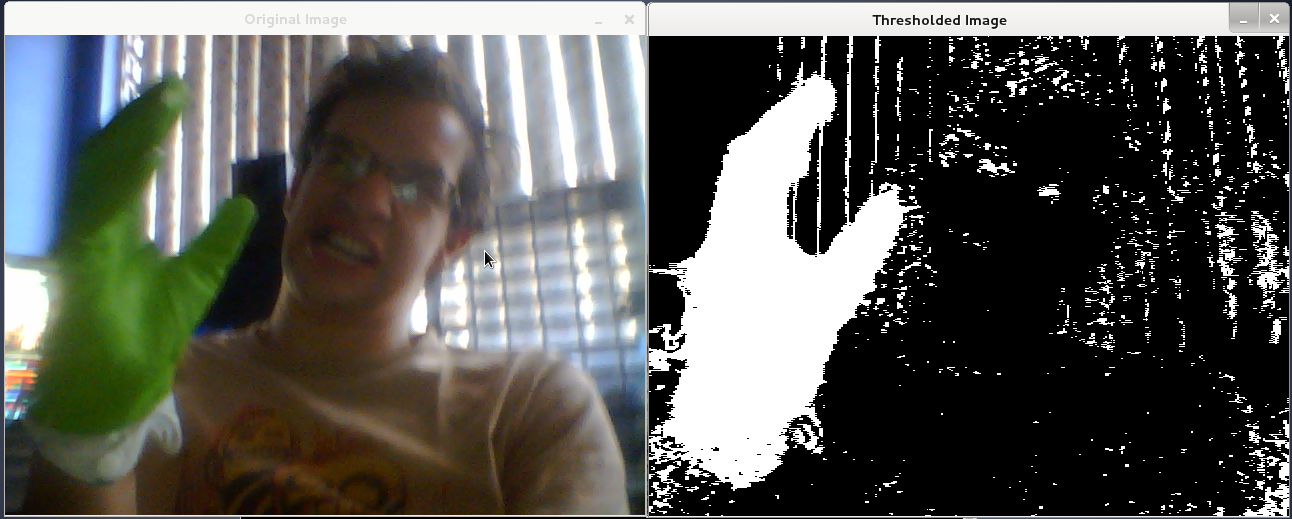
\includegraphics[scale=0.25]{pic02.png}
\end{center}
\end{frame}
%%*****************************************************************************
\begin{frame}
\frametitle{Pre-processing-Final}
\begin{center}
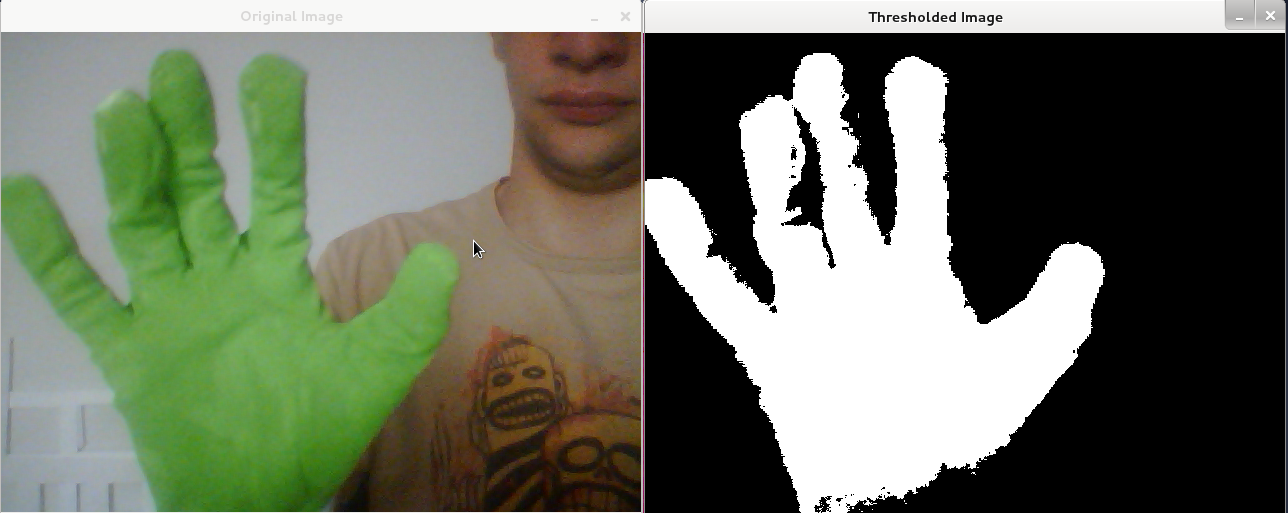
\includegraphics[scale=0.25]{pic03.png}
\end{center}
\end{frame}
%%*****************************************************************************
\begin{frame}
\frametitle{Tasks of computer vision}
\begin{itemize}
\item Simple Object-Color recognition
\item Tracking 
\end{itemize}
\end{frame}
%%*****************************************************************************
\section{Implementation}
\begin{frame}
\frametitle{Example 1}
Entertainment on EIE\\
\begin{center}
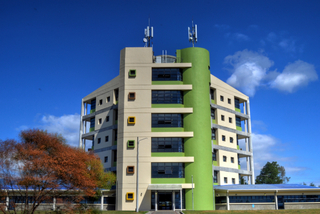
\includegraphics[scale=0.6]{edificio.jpg}
\end{center}
\end{frame}
%%*****************************************************************************
\begin{frame}
\frametitle{Example 2}
Interactive banners on bus stops\\
\begin{center}
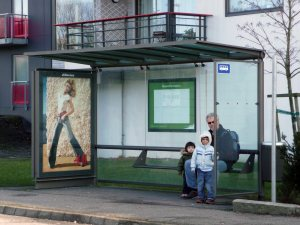
\includegraphics[scale=1]{bus_stop.jpg}
\end{center}
\end{frame}
%%*****************************************************************************
\section{Prototype}
\begin{frame}
\frametitle{Pong}
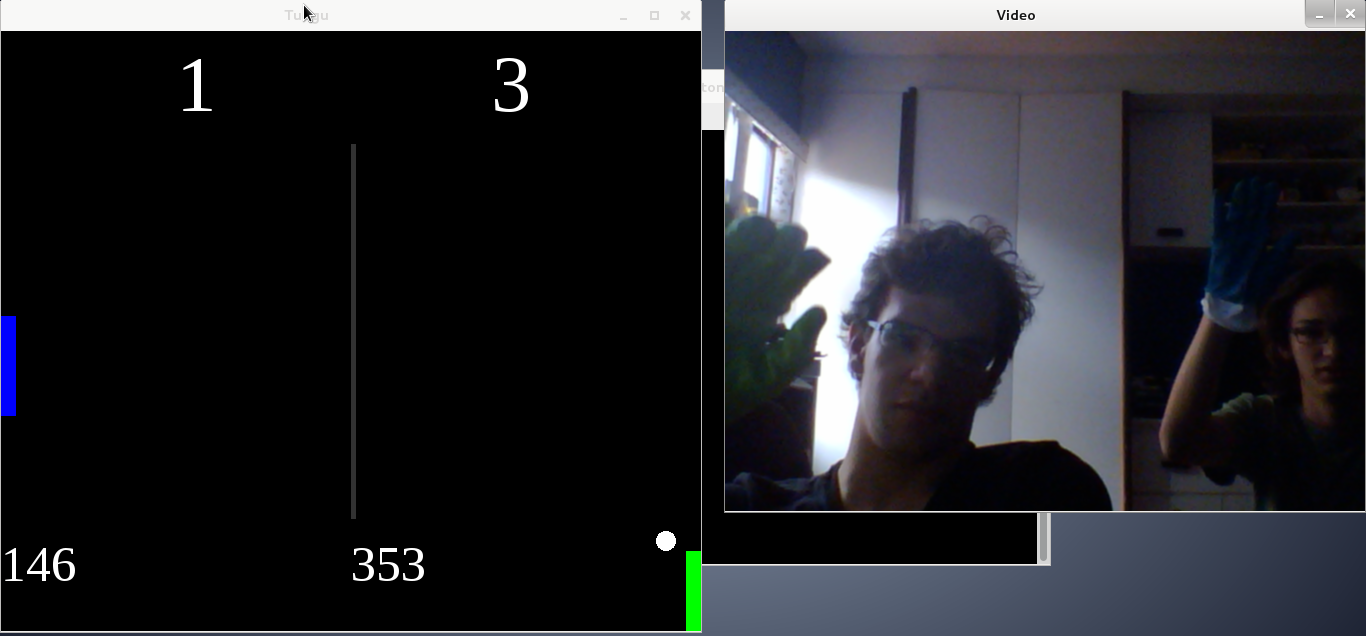
\includegraphics[scale=0.24]{picpong.png}
\end{frame}
%%*****************************************************************************
\begin{frame}
\frametitle{Demo}
\end{frame}
%%*****************************************************************************
\section{Conclusion \& Questions}
\begin{frame}
 \frametitle{Conclusion}
\begin{itemize}
\item It would be a great solution 
\item The lib opencv allows you a wide range of posibilities
\item Understanding how Visual processing works for entertainment
\item Gesture recognition is another form of comunication with technology
 
%\item Documentation
\end{itemize}
%Moose
%fork
\end{frame}
%%*****************************************************************************
\begin{frame}
 \frametitle{Questions?}
\end{frame}
%%*****************************************************************************

\end{document}
